\chapter{Thực nghiệm và đánh giá kết quả}
\ifpdf
    \graphicspath{{Chapter4/Chapter4Figs/PNG/}{Chapter4/Chapter4Figs/PDF/}{Chapter4/Chapter4Figs/}}
\else
    \graphicspath{{Chapter4/Chapter4Figs/EPS/}{Chapter4/Chapter4Figs/}}
\fi
\markboth{\MakeUppercase{\thechapter. Các bộ dữ liệu và phương thức đánh giá}}{\thechapter. Các bộ dữ liệu và phương thức đánh giá}

Chương này sẽ trình bày...

\section{Các bộ dữ liệu và phương thức đánh giá}
Mục này sẽ trình bày quy trình đánh giá chuẩn được sử dụng rộng rãi trong truy vấn đối tượng trên tập dữ liệu lớn. Trước tiên là mô tả về các bộ dữ liệu chuẩn, sau đó là phần trình bày chi tiết về phương thức đánh giá cho các kết quả thí nghiệm.

\subsection{Các bộ dữ liệu}

\subsubsection{Oxford 5k}
Bộ dữ liệu Oxford 5k được xây dựng bởi \cite{philbin2007object}, bao gồm 11 Oxford "landmark"\footnote{landmark ở đây có nghĩa là một góc nhìn/góc chụp đặc biệt của một tòa nhà} cùng các hình ảnh gây nhiễu. Hình ảnh cho mỗi landmark được tự động lấy về từ trang chia sẻ ảnh trực tuyến Flickr sử dụng các câu truy vấn như "Oxford Christ Church" và "Oxford Radcliffee Camera", đồng thời các hình ảnh gây nhiễu cũng được lấy về bằng câu truy vấn "Oxford". Bộ dữ liệu bao gồm 5,062 hình ảnh chất lượng cao (1366 $\times$ 768).\\
\textit{Tập dữ liệu đánh giá chuẩn} (ground truth) được xây dựng thủ công cho 11 landmark. Các hình ảnh được gán vào một trong bốn nhãn: \textit{Good} nếu nó là một hình ảnh rõ ràng và đầy đủ về đối tượng/tòa nhà, \textit{OK} nếu hình ảnh chứa hơn 25\% của đối tượng và \textit{Junk} nếu hình ảnh chứa ít hơn 25\% của đối tượng hoặc đối tượng bị che khuất phần lớn hoặc hình ảnh đối tượng bị méo mó nhiều.\\
Bộ dữ liệu gồm 55 truy vấn trong đó mỗi landmark sẽ có 5 truy vấn. Các đối tượng sẽ được khoanh vùng trên các hình ảnh truy vấn. Tất cả các truy vấn được thể hiện trong hình \ref{FigOxfordDataset}.

\begin{figure}[!htbp]
  \begin{center}
    \leavevmode
    \ifpdf
      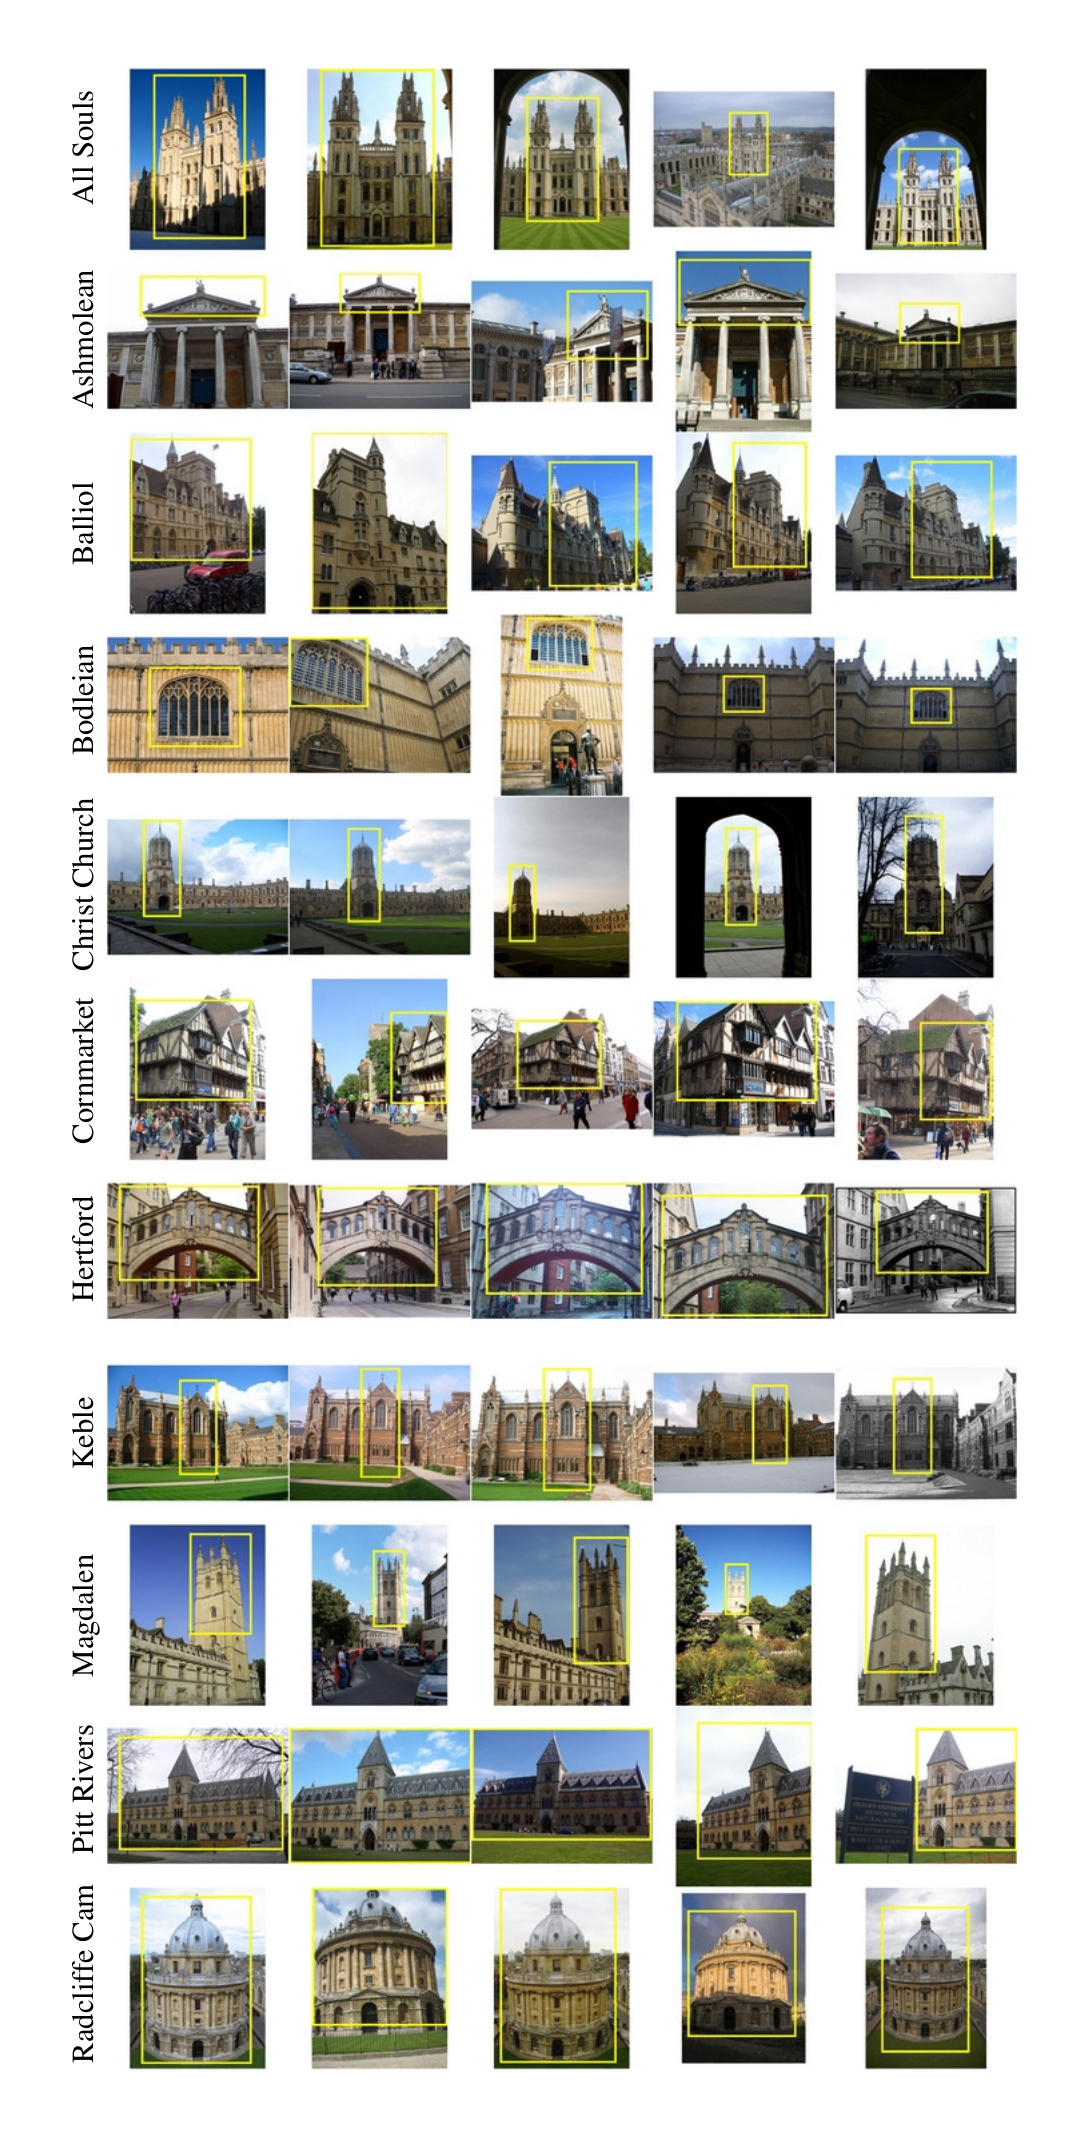
\includegraphics[scale=0.27]{oxfordDataset}
    \else
      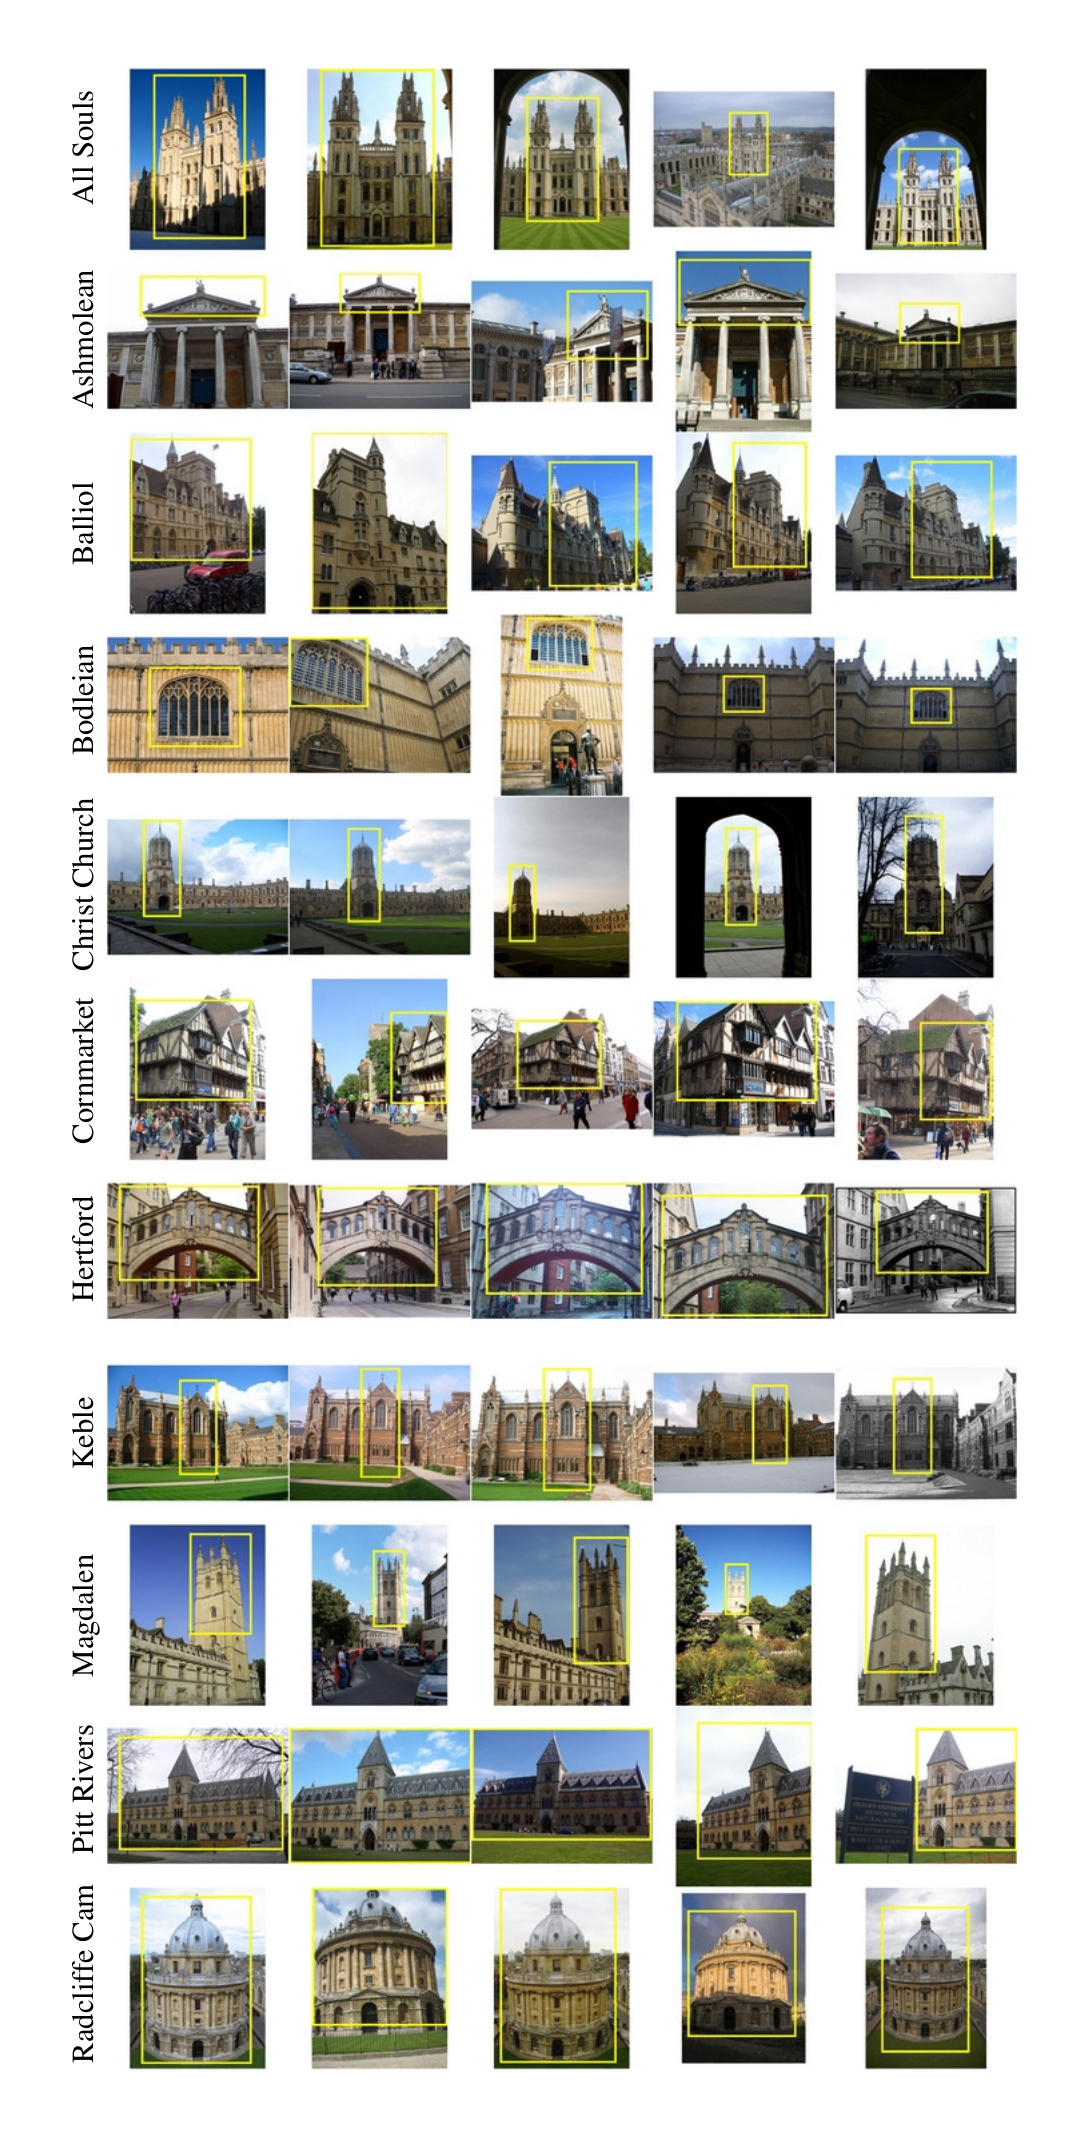
\includegraphics[scale=0.27]{oxfordDataset}
    \fi
    \caption[Landmark và các truy vấn được dùng để đánh giá]{\textbf{Landmark và các truy vấn được dùng để đánh giá} 55 hình ảnh truy vấn được sử dụng trong tập dữ liệu đánh giá chuẩn. Mỗi hàng là 5 hình của 5 truy vấn khác nhau cho cùng một cảnh landmark. Hình ảnh được lấy từ bài báo \citep{philbin2007object}.}
    \label{FigOxfordDataset}
  \end{center}
\end{figure}

\subsubsection{Paris 6k}
Tương tự như bộ dữ liệu Oxford 5k, Paris 6k bao gồm 6,392 hình ảnh chất lượng cao (1366 $\times$ 768) của các địa danh nổi tiếng ở Paris được lấy về từ Flickr với các câu truy vấn như "Paris Eiffel Tower" hay "Paris Triomphe". Paris 6k cũng có 55 hình ảnh truy vấn cho 11 landmark (5 truy vấn cho mỗi landmark) (\cite{philbin2008lost}).\\
Paris 6k được đánh giá là một bộ dữ liệu hoàn toàn độc lập so với Oxford 5k và thường được dùng để kiểm tra các tác động của việc tính toán từ trực quan trong khi Oxford 5k thường được dùng để kiểm tra hiệu suất.\\

\subsubsection{Holidays}
Bộ Holidays bao gồm 1,491 hình ảnh chất lượng cao về các lễ hội với 500 truy vấn mà mỗi truy vấn chứa một vài hình ảnh chính xác về đối tượng truy vấn (\cite{JDS08}). Bộ dữ liệu này nhằm hướng tới mục đích truy vấn ảnh trên tập dữ liệu lớn vì các hình ảnh không phải về một đối tượng đặc biệt như trong Oxford 5k và Paris 6k, đồng thời các thay đổi trên hình ảnh của đối tượng cũng đa dạng hơn với nhiều loại thay đổi khác nhau và truy vấn được thực hiện với toàn bộ hình ảnh chứ không phải với một vùng hình ảnh có chứa đối tượng được chỉ định trước.\\
Tập dữ liệu bao gồm 500 nhóm hình ảnh, mỗi nhóm là một cảnh khác nhau và bao gồm rất nhiều loại hình ảnh khác nhau như tự nhiên, nhân tạo, hiệu ứng nước và lửa,... Hình ảnh đầu tiên của mỗi nhóm là hình truy vấn và các hình còn lại trong nhóm là kết quả chính xác cho truy vấn. Và các hình ảnh truy vấn không được xem xét tới trong kết quả trả về chứ không phải được xem là một kết quả chính xác như trong Oxford 5k và Paris 6k.\\
Thông thường bô dữ liệu Holidays thường được ghép với khoảng 1 triệu hình ảnh từ Flickr khác để kiểm tra truy vấn trên tập dữ liệu lớn, thường được gọi là bộ dữ liệu \textit{Holidays + Flickr1M}.\\

\subsection{Phương thức đánh giá}
\label{evaluation}
Với mỗi truy vấn, để đánh giá kết quả trả về ta thường dùng độ đo \textit{precision-recall} (PR). Precision là tỉ lệ giữa số kết quả đúng trả về trong tổng số kết quả trả về. Recall là tỉ số của số kết quả đúng trả về trên tổng số hình ảnh đúng trong tập dữ liệu. Hay nói theo cách khác, precison cho thấy độ "tinh khiết" của kết quả trả về, còn recall cho biết đã tìm thấy bao nhiêu phần của đáp án.\\
Tùy theo từng mục đích mà người ta sẽ tập trung vào việc nâng cao precision hay recall. Ví dụ, những ứng dụng như Google Goggles\footnote{Google Goggles là một ứng dụng nhận dạng hình ảnh được phát hành bởi Google. Người sử dụng điện thoại di động chỉ cần chụp ảnh của đối tượng như xe hơi, đồ chơi, bìa sách, mã vạch,... sau đó Goggles sẽ quét và đối chiếu kho dữ liệu để hiển thị thông tin liên quan đến vật đó.} thì câu hỏi nó cần phải trả lời là "Nó là cái gì?", do đó nó chỉ chú ý đến việc đạt được chỉ số precison tối đa có thể, tức là lấy được những kết quả đúng nhưng vừa đủ để nhận dạng đối tượng. Trong nhiều trường hợp khác thì chỉ số recall cũng được quan tâm. Ví dụ việc tái tạo không gian ba chiều đòi hỏi phải tìm được đủ số lượng hình ảnh của đối tượng để xây dựng được mô hình ba chiều chính xác.\\
Để đo hiệu suất thực thi của hệ thống, ở đây ta dùng độ đo average precision (AP)(\cite{philbin2007object}), nó cũng tương đương với phần diện tích bên dưới đường biểu diễn cho chỉ số precision-recall trong biểu đồ. Một đường biểu diễn precision-recall lý tưởng có chỉ số precision bằng 1 trên tất cả các mức recall khác nhau và nó tương ứng chỉ số average precision bằng 1. Average precision được tính cho từng truy vấn một sau đó ta lấy trung bình cộng của chúng, đó chính là mean Average Precision - một con số để đánh giá hiệu suất tổng thể của hệ thống.

\section{Cài đặt thí nghiệm}
Lorem ipsum dolor sit amet, consectetur adipiscing elit. Vestibulum euismod libero a augue suscipit, a dignissim justo ullamcorper. Nunc in tincidunt dolor, sed feugiat ante. Curabitur ut elit sit amet dui euismod congue porttitor rhoncus enim. Donec in mollis massa, et sagittis est. Duis est dui, suscipit id sollicitudin vel, malesuada non metus. Vivamus tincidunt libero non nunc dignissim, interdum auctor lorem lacinia. Praesent ultrices nec turpis placerat consectetur. Maecenas volutpat lobortis interdum. Fusce ullamcorper nunc at varius bibendum. Praesent at ipsum sagittis, facilisis leo ac, commodo orci.

Proin eu velit semper, molestie ipsum sit amet, consequat quam. Fusce rhoncus est in facilisis mattis. Pellentesque habitant morbi tristique senectus et netus et malesuada fames ac turpis egestas. Vivamus accumsan, erat sed egestas luctus, orci turpis posuere dolor, ut tempor magna enim et mauris. Maecenas in scelerisque quam, id bibendum lacus. Nullam rutrum odio id magna porttitor tincidunt. Cum sociis natoque penatibus et magnis dis parturient montes, nascetur ridiculus mus. Aliquam feugiat elit sapien, eget consectetur sapien tempor et. Aenean tempus eleifend laoreet. Vivamus nec mollis orci. Maecenas sit amet quam nibh. Phasellus blandit fringilla massa faucibus porta. Fusce mattis pellentesque leo, sed auctor mi lobortis viverra. Donec sed arcu non orci gravida accumsan nec in diam. Proin malesuada enim sed est sagittis, tincidunt sollicitudin metus suscipit. Vivamus dapibus suscipit diam, fringilla fermentum arcu dignissim eu.

Aliquam eget velit vitae ligula pharetra malesuada. Maecenas ut facilisis lorem, in dapibus dolor. Curabitur pulvinar dolor a adipiscing dignissim. Maecenas sed porttitor ligula. Morbi vitae lacus laoreet, posuere odio eget, vehicula dui. Pellentesque lectus metus, rutrum vulputate nisl et, consequat rutrum augue. Fusce mollis dolor vitae lectus commodo ornare. Sed volutpat in magna ut mollis. Maecenas sodales tincidunt iaculis. Interdum et malesuada fames ac ante ipsum primis in faucibus. Interdum et malesuada fames ac ante ipsum primis in faucibus. Proin ut aliquam lorem. Suspendisse adipiscing lacinia dictum. Morbi at augue id mauris imperdiet tincidunt eu sit amet elit.

\section{Kết quả thí nghiệm và đánh giá kết quả}
Lorem ipsum dolor sit amet, consectetur adipiscing elit. Aenean tincidunt risus eros, ac molestie quam lobortis at. Proin ante dolor, lacinia vel risus cursus, commodo rutrum lacus. Donec dapibus euismod sollicitudin. Sed viverra sapien tempor velit pulvinar, a condimentum quam aliquam. Vivamus purus purus, sagittis eu bibendum in, vulputate nec magna. Aliquam erat volutpat. Nulla facilisi.

Sed porta elit in vehicula pellentesque. Morbi faucibus mollis libero, ac volutpat lectus sagittis ut. Vestibulum eget fermentum eros. Suspendisse potenti. Nunc ac luctus nunc, id dapibus dolor. Curabitur lorem ante, pretium et nunc nec, iaculis laoreet metus. Pellentesque vitae nisi id magna pulvinar pulvinar. Quisque venenatis dolor sit amet velit elementum tincidunt. Sed purus dui, varius in dui eget, mollis venenatis lacus. Fusce vestibulum metus eget mauris accumsan varius. Donec dapibus iaculis cursus. Duis ut congue diam. Quisque convallis mi sodales, condimentum nisi nec, consequat lectus. Integer posuere venenatis hendrerit.
